\documentclass{bredelebeamer}


\begin{document}

\title[INFO-F-410 - Traffic Light Control]{\textbf{Traffic Light Control} \\INFO-F-410 -- Embedded Systems Design} % The short title appears at the bottom of every slide, the full title is only on the title page

\author{Jamal \textsc{Ben Azouze}, Marien \textsc{Bourguignon}, Nicolas \textsc{De Groote}, \\Simon \textsc{Picard}, Arnaud \textsc{Rosette}, Gabriel \textsc{Ekanga}}
\institute[ULB] % Your institution as it will appear on the bottom of every slide, may be shorthand to save space
{
Université Libre de Bruxelles \\ % Your institution for the title page
\medskip
\textit{Département d'Informatique} % Your email address
}
\date{4 Juin 2015} % Date, can be changed to a custom date

\begin{frame}
\titlepage % Print the title page as the first slide
\end{frame}

\begin{frame}{Sommaire}
\tableofcontents % Throughout your presentation, if you choose to use \section{} and \subsection{} commands, these will automatically be printed on this slide as an overview of your presentation
\end{frame}

\section{Introduction}
\begin{frame}{Introduction}

\end{frame}

\section{Acteurs et automates}
\begin{frame}{Acteurs et automates}

\end{frame}

\section{Winning condition}
\begin{frame}[fragile]{Winning condition}
\begin{alertblock}{}
Pure safety : the controler \textbf{must} avoid the losing states.
\begin{verbatim}
control : A[] not(lose)
\end{verbatim}
\end{alertblock}



\begin{block}{1. A pedestrian is never knocked down}
\begin{verbatim}
form_1 = 
control: A[] not(PedestrianGeneratorEast.Cross && 
(
    CarGeneratorEast.Go || 
    (
        CarGeneratorWest.Go && queue[W][0] == U
    ) || (
        CarGeneratorSouth.Go && queue[S][0] == R
    )))
\end{verbatim}
\end{block}

\end{frame}
\begin{frame}[fragile]{Winning condition}
\centering
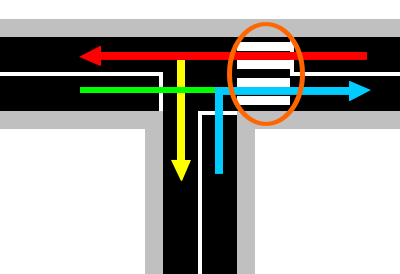
\includegraphics[scale=0.8]{images/pietonCollision.png}

\end{frame}


\begin{frame}[fragile]{Winning condition}
\begin{block}{2. Cars should never collide}
\begin{verbatim}
form_2 = 
Control: A[] not
(
    CarGeneratorWest.Go && queue[W][0] == U && 
    ((
        CarGeneratorEast.Go && queue[E][0] == L
    ) || (
        CarGeneratorSouth.Go && 
        ( queue[S][0] == L || queue[S][0] == R )
    ))
) || (
    CarGeneratorWest.Go && queue[W][0] == R 
    && CarGeneratorEast.Go && queue[E][0] == L
)
\end{verbatim}

Same idea for the two other orientations.
\end{block}

\end{frame}
\begin{frame}[fragile]{Winning condition}
\centering
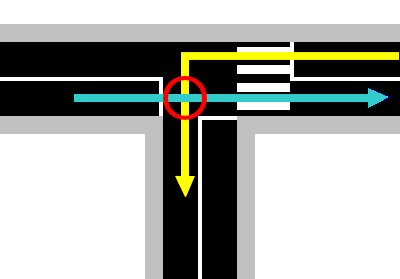
\includegraphics[scale=0.8]{images/exempleCollision.png}

\end{frame}


\begin{frame}[fragile]{Winning condition}
\begin{block}{3. Pedestrians do not wait infinitely}
\begin{verbatim}
form_3 = 
control: A[] not (PedestrianGeneratorEast.Broken)
\end{verbatim}
\end{block}

\begin{block}{4. Cars do not wait infinitely}
\begin{verbatim}
form_4 = 
control: A[] not (CarGeneratorEast.Broken ||
                  CarGeneratorSouth.Broken ||
                  CarGeneratorWest.Broken)
\end{verbatim}
\end{block}
\begin{block}{Full condition}
\begin{verbatim}
control: A[] not (
    form_1 || form_2 || form_3 ||form_4
)
\end{verbatim}
\end{block}
\end{frame} 

\section{Simulation}
\begin{frame}{Simulator}

\begin{block}{Base idea}
\begin{itemize}
\item Illustrate controller-environment interactions 
\item Environment behaves randomly
\item Controller avoids the bad states by implementing a winning strategy
\end{itemize}
\end{block}

\begin{block}{Problems}

\begin{itemize}
\item The winning strategy is huge ! 
\item It specifies a transition of the controller from each system state. 
\item Generate an execution trace from Uppaal tiga does not work (software problem)
\end{itemize}

\end{block}

\end{frame}

\begin{frame}{Simulator}

\begin{block}{Solution }
\begin{itemize}
\item Define a controller following a winning strategy in Uppaal (not tiga)
\item Then generate a trace of the whole system. 
\item Finally, convert this trace via the Libutap library (readable)
\end{itemize}
\end{block}

\begin{block}{GUI}
\begin{itemize}
\item Cars (bleu arrow), car lights (red arrow)
\item Pedestrians (yellow arrow), pedestrian light (green arrow)
\end{itemize}

\end{block}



\end{frame}

\begin{frame}{Simulator}

\centering
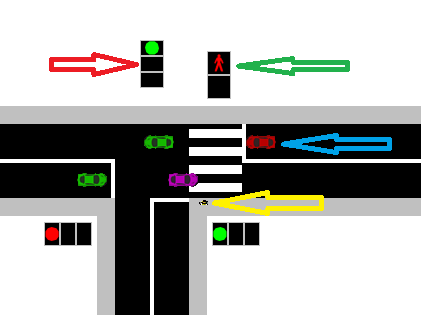
\includegraphics[scale=0.8]{images/SimP.png}

\end{frame}


\section{Conclusion}
\begin{frame}{Conclusion}

\end{frame}
\end{document}
